% Тут используется класс, установленный на сервере Papeeria. На случай, если
% текст понадобится редактировать где-то в другом месте, рядом лежит файл matmex-diploma-custom.cls
% который в момент своего создания был идентичен классу, установленному на сервере.
% Для того, чтобы им воспользоваться, замените matmex-diploma на matmex-diploma-custom
% Если вы работаете исключительно в Papeeria то мы настоятельно рекомендуем пользоваться
% классом matmex-diploma, поскольку он будет автоматически обновляться по мере внесения корректив
%

% По умолчанию используется шрифт 14 размера. Если нужен 12-й шрифт, уберите опцию [14pt]
\documentclass[14pt]{matmex-diploma-custom}
%\documentclass[14pt]{matmex-diploma-custom}

\begin{document}
%\graphicspath{/images} 
% Год, город, название университета и факультета предопределены,
% но можно и поменять.
% Если англоязычная титульная страница не нужна, то ее можно просто удалить.
\filltitle{ru}{
    chair              = {Кафедра системного программирования},
    title              = {Workflow Builder для библиотеки Brahma.FSharp},
    % Здесь указывается тип работы. Возможные значения:
    %   coursework - Курсовая работа
    %   diploma - Диплом специалиста
    %   master - Диплом магистра
    %   bachelor - Диплом бакалавра
    type               = {coursework},
    position           = {студента},
    group              = 243,
    author             = {Васенина Анна Игоревна},
    supervisorPosition = {магистр ИТ, ст. преп.},
    supervisor         = {Григорьев С.В.},
%   university         = {Санкт-Петербургский Государственный Университет},
%   faculty            = {Математико-механический факультет},
%   city               = {Санкт-Петербург},
%   year               = {2013}
}
\maketitle
\tableofcontents
% У введения нет номера главы
\section*{Введение}
Cегодня вычисления на графическом процессоре (GPU) становятся всё более популярными, связано это с увеличением объема вычисляемых данных и необходимостью параллельного вычисления для эффективной их обработки. Одной из распространенных технологий для программирования на GPU является OpenCL~(\cite{OpenCL}), основным преимуществом которой является возможность работы на любых устройствах, поддерживающих данный стандарт .

Стандарт OpenCL реализован для множества языков программирования, таких как Python, Java. Реализацией стандарта OpenCL для языка F\# стала библиотека Brahma.FSharp~(\cite{Brahma}).

К сожалению, на данный момент в этой библиотеке существует ряд проблем. Одна из них - это неудобство явной передачи контекста как с точки зрения программиста при написании кода, так и с точки зрения реализации последовательных операций с одним элементом.

Сейчас работа с элементами в библиотеке Brahma осуществляется по схеме, изображенной на рис. 1
% Рисунок, размещенный с предпочтением "вверху страницы"
\begin{figure}[h] 
\label{13}
\centering 
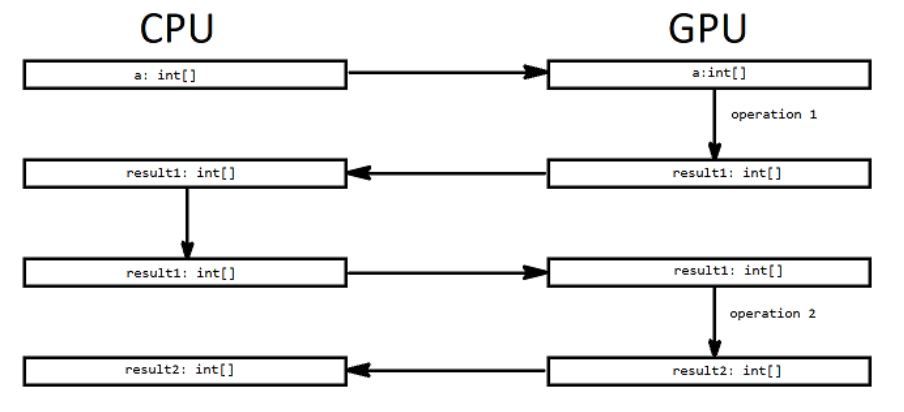
\includegraphics[width=0.9\textwidth]{images/pic1} 
\caption{Диаграмма модулей} 
\end{figure}

Такая схема работы требует улучшения, потому что:
Пользователю неудобно в явном виде пересылать контекст на каждом шаге
Замедляется работа программы из-за пересылок
Удобство написания кода в библиотеке имеет не малое значение для программиста, использующего её. Поэтому необходимо давать как можно более удобные механизмы работы для того, чтобы пользователь был доволен библиотекой и предпочитал использовать именно её. Неявная передача контекста позволяет пользователю избежать возможных ошибок при манипуляциях с контекстом.

Возможность последовательно выполнять операции с одним массивом на GPU, не возвращая каждый раз массив не менее важна, так как обычно нам приходится иметь дело с небольшим количеством исходных массивов, над которыми нужно провести множество операций, а возвращая после каждой операции массив обратно в CPU, мы проигрываем не только в красоте и читаемости кода, но и в скорости выполнения операций.


\section{Обзор}
Для решения данных проблем было решено создать workflow builder. Средствами создания его выступили монада reader и computation expressions.
\subsection {Brahma.FSharp}
Brahma.Fsharp нацелена на трансляцию кода на FSharp в OpenCL с минимизацией различных пользовательских типов и врапперов.
Данная библиотека предоставляет пользователю следующие возможности:
\begin{itemize}
\item использование OpenCL для работы на GPU с любыми устройствами, которые поддерживают OpenCL, например с устройствами AMD и Nvidia;
\item поддерживает кортежи и структуры;
\item использование строго типизированных ядер из OpenCL.
\end{itemize}
\subsection {Монады и монада reader}~(\cite{habrahabr})
Монада это конструкция функционального программирования, которая позволяет применить функцию, возвращающую упакованное значение к упакованному значению.
Монада reader (см. рис.2)~(\ref{reader}) позволяет нам неявно передать какие-то настройки в функцию неявно, скрывая сам процесс передачи этих настроек за кулисами. Она организовывает упаковку функции в контекст и его распаковку для применения функции. Монаду характеризуют функции bind (>>=) для соединения содержательной части с контекстом и run для их отделения.
\begin{figure}[h] 
\label{reader}
\centering 
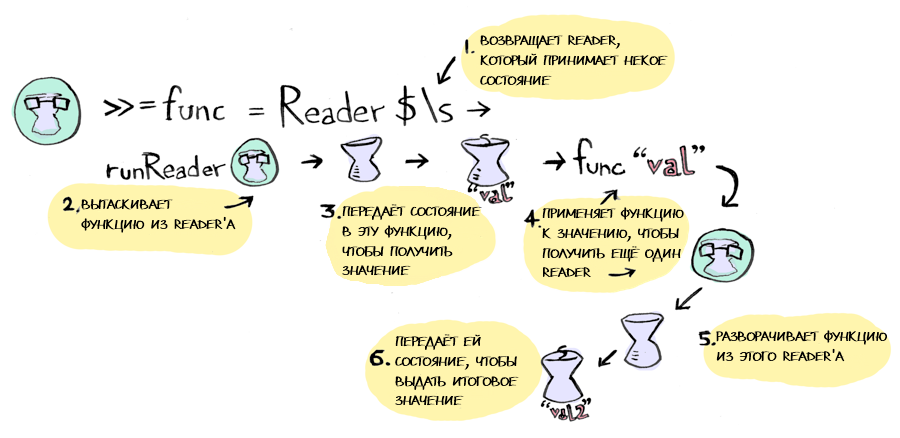
\includegraphics[width=0.9\textwidth]{images/reader} 
\caption{Рис. 2 Схематичная работа монады Reader
Источник: \url{https://habrahabr.ru/post/184722/}
} 
\end{figure}
\subsection{Computation expressions}~(\cite{fsffap})
По сути своей сomputation expressions представляют некую именованную среду, ограниченную фигурными скобками (например, gpu\{\ldots\}), для которой мы переопределяем ключевое слово let! необходимым нам образом, а так же определяем другие ключевые слова, такие как return. 
Каждый computation expression работает с некоторым типом-оберткой, именно его мы и используем для упаковки контекста и содержательной составляющей данных.

\section{Постановка задачи}
При написании данной работы преследовалось две основные цели:
\begin{itemize}
    \item повысить удобство написания кода для пользователя путем   неявной передачи в функции заданный в начале работы контекст;
\item возможность выполнять последовательно операции с  массивами на GPU, не    возвращая массив каждый раз после исполнения функции.   
\end{itemize}
Для их выполнения были поставлены следующие задачи:
\begin{itemize}
    \item Реализовать модуль \verb|gpu{...}| и конструктор таких модулей для разных контекстов. Внутри которых происходит работа с одним контекстом, передающимся выполняемым функциям неявно.
    \item Протестировать данный модуль на нескольких примерах с использованием функций массивов из модуля ArrayGPU, снабдить их комментариями.
\end{itemize}

\section{Решение}
Для решения поставленной задачи был создан специальный тип  
ReaderM <’d,’out> являющийся оберткой для нашего computation expression. Также необходимо было научить работать данный computation с этим типом. Для этого были применены методы монады reader: bind для переопределения ключевого слова let! и constant для того, чтобы обернуть значение при вызове функций return и yield. Reader.run явно вызывается только после получения результата computatuion’а для того, чтобы отделить нужные данные от контекста.

Благодаря функции bind мы больше не должны манипулировать контекстом: внутри модуля gpu получаем следующую ротацию типов.
\begin{figure}[h] 
\label{table}
\centering 
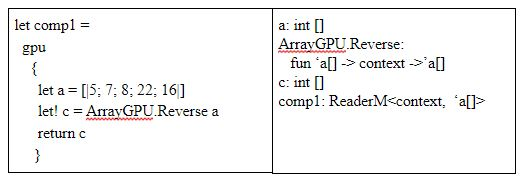
\includegraphics[width=0.9\textwidth]{images/types} 
\end{figure}

Как можно видеть, модуль gpu решает вопрос неявной передачи контекста для удобства пользователя.

Контекст, который передается функциям, монада reader берет первый подходящий, который она встретит в модуле. 
Однако, при этом все равно необходимо передавать контекст в билдер для того, чтобы не пришлось вручную переводить массив на CPU при выполнении функции return, а также очищать буфера и сбрасывать очередь команд после завершения работы - команда return сделает это за пользователя.

Однако, нам необходимо иметь также возможность вернуться из композиции computation’ов, не проводя манипуляций с контекстом. Для этого мы используем метод Yield, который так же, как и return использует функцию constant для того, чтобы обернуть результат типом ReaderM <’d,’out>, но не очищает буфера и не сбрасывает очередь команд.
Благодаря этому мы получаем возможность построения таких конструкций:
\begin{verbatim}
let x = 1
\end{verbatim}

\begin{figure}[h] 
\label{code}
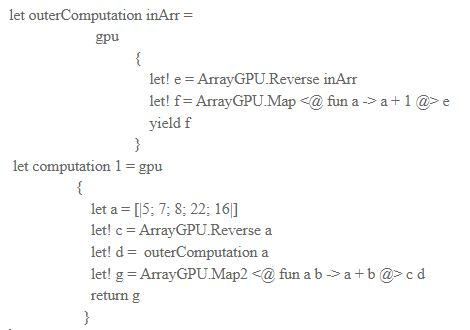
\includegraphics[width=0.9\textwidth]{images/code} 
\end{figure}

Для того, чтобы использовать метод yield необходимо определить метод Zero, который говорит, какое значение присвоить всему выражению, если computation пытается вернуть тип unit. В данном решении мы определили, что computation должен вернуть обернутый None.

% У заключения нет номера главы
\section*{Заключение}
В ходе работы получены следующие результаты:
\begin{itemize}
    \item реализована возможность выполнения последовательных операций на GPU;
    \item внутри модуля gpu{..} производится работа с заранее определенным       контекстом вида (ComputeProvider * CommandQueue * int * int). Работать с функциями получающими такой контекст последним из аргументов можно без указания контекста.
\end{itemize}

В качестве дальнейшего развития можно рассмотреть следующее направление: в некоторых случаях возникает необходимость работать в разных контекстах с одними данными. На данный момент работа с разными контекстами не поддерживается, но в рамках workflow builder’а это можно реализовать при использовании композиции нескольких computation expressions (например, gpu1{..} и gpu2{..}), каждый из которых работает со своим контекстом. 

\setmonofont[Mapping=tex-text]{CMU Typewriter Text}
\bibliographystyle{ugost2008ls}
\bibliography{diploma.bib}
\end{document}
